
\documentclass[12pt]{article}

% Layout.
\usepackage[top=1in, bottom=0.75in, left=1in, right=1in, headheight=1in, headsep=6pt]{geometry}

% Fonts.
\usepackage{mathptmx}
\usepackage[scaled=0.86]{helvet}
\renewcommand{\emph}[1]{\textsf{\textbf{#1}}}

% TiKZ.
\usepackage{tikz, pgfplots}
\usetikzlibrary{calc}
\pgfplotsset{compat = newest}
 
\pgfplotsset{my style/.append style={axis x line=middle, axis y line=
middle, xlabel={$x$}, ylabel={$y$}, axis equal }}

% Misc packages.
\usepackage{amsmath,amssymb,latexsym}
\usepackage{graphicx}
\usepackage{array}
\usepackage{xcolor}
\usepackage{multicol}

% Commands to set various header/footer components.
\makeatletter
\def\doctitle#1{\gdef\@doctitle{#1}}
\doctitle{Use {\tt\textbackslash doctitle\{MY LABEL\}}.}
\def\docdate#1{\gdef\@docdate{#1}}
\docdate{Use {\tt\textbackslash docdate\{MY DATE\}}.}
\def\doccourse#1{\gdef\@doccourse{#1}}
\let\@doccourse\@empty
\def\docscoring#1{\gdef\@docscoring{#1}}
\let\@docscoring\@empty
\def\docversion#1{\gdef\@docversion{#1}}
\let\@docversion\@empty
\makeatother

% Headers and footers layout.
\makeatletter
\usepackage{fancyhdr}
\pagestyle{fancy}
\fancyhf{} % Clears all headers/footers.
\lhead{\baselineskip 30pt
%\emph{\@doctitle\hfill\@docdate}
\emph{\@docdate\hfill\@doctitle}
\ifnum \value{page} > 1\relax\else\\
\emph{Name: \rule{3.5in}{1pt}\hfill \@docscoring}\fi}
\rfoot{\emph{\@docversion}}
\lfoot{\emph{\@doccourse}}
\cfoot{\emph{\thepage}}
\renewcommand{\headrulewidth}{0pt}%
\makeatother

% Paragraph spacing
\parindent 0pt
\parskip 6pt plus 1pt

% A problem is a section-like command. Use \problem{5} to
% start a problem worth 5 points.
\newcounter{probcount}
\newcounter{subprobcount}
\setcounter{probcount}{0}
\newcommand{\problem}[1]{%
\par
\addvspace{4pt}%
\setcounter{subprobcount}{0}%
\stepcounter{probcount}%
\makebox[0pt][r]{\emph{\arabic{probcount}.}\hskip1ex}\emph{[#1 points]}\hskip1ex}
\newcommand{\thesubproblem}{\emph{\alph{subprobcount}.}}

% Subproblems are an enumerate-like environment with a consistent
% numbering scheme. 
% Use \begin{subproblems}\item...\item...\end{subproblems}
\newenvironment{subproblems}{%
\begin{enumerate}%
\setcounter{enumi}{\value{subprobcount}}%
\renewcommand{\theenumi}{\emph{\alph{enumi}}}}%
{\setcounter{subprobcount}{\value{enumi}}\end{enumerate}}

% Blanks for answers in normal and math mode.
\newcommand{\blank}[1]{\rule{#1}{0.75pt}}
\newcommand{\mblank}[1]{\underline{\hspace{#1}}}
\def\emptybox(#1,#2){\framebox{\parbox[c][#2]{#1}{\rule{0pt}{0pt}}}}

% Misc.
\renewcommand{\d}{\displaystyle}
\newcommand{\ds}{\displaystyle}
\def\bc{\begin{center}}
\def\ec{\end{center}}
\def\be{\begin{enumerate}}
\def\ee{\end{enumerate}}


\doctitle{Math 251: Quiz 2}
\docdate{Jan 19, 2022}
\doccourse{UAF Calculus I}
\docversion{v-1}
\docscoring{\blank{0.8in} / 25}
\begin{document}
%\textbf{Please circle your instructor's name:} \hfill Leah Berman  \hfill   Jill Faudree\\

There are 25 points possible on this quiz. No aids (book, calculator, etc.)
are permitted.  {\bf Show all work for full credit.}

\problem{11} Let $P(0,6)$ be a point on the graph of $f(x)=\displaystyle{\frac{10}{x+1}+x-4}.$
\begin{subproblems}
\item Find the slope of the secant line passing through $P$ and the point $Q(1,f(1)).$ 
\vfill

\item Find the slope of the secant line passing through $P$ and the point $Q(4,f(4)).$

\vfill

\item The table below lists the slope of the secant line passing through the point $P$ and the point $Q(x, f(x))$ for several values of $x.$ \\

\begin{tabular}{l || c|c|c|c|c|c}
x&-0.1&-0.01&-0.001&0.001&0.01&0.1\\
\hline
f(x)&7.011111&6.091010&6.00901&5.99910&5.9910 &5.91099 \\
\hline
$m_{sec}$&-10.111111 &-9.101010&-9.00100&-8.99900&-8.90099&-8.090909\\
\end{tabular}

\vskip 0.5cm
Use the information in the table to estimate the slope of the tangent line to $f(x)$ at the point $P(0,6).$
\vfill


\item Use the slope from part (c) above to write an equation of the tangent line at point $P(0,6).$

\vfill

\item \quad 

\begin{multicols}{2}
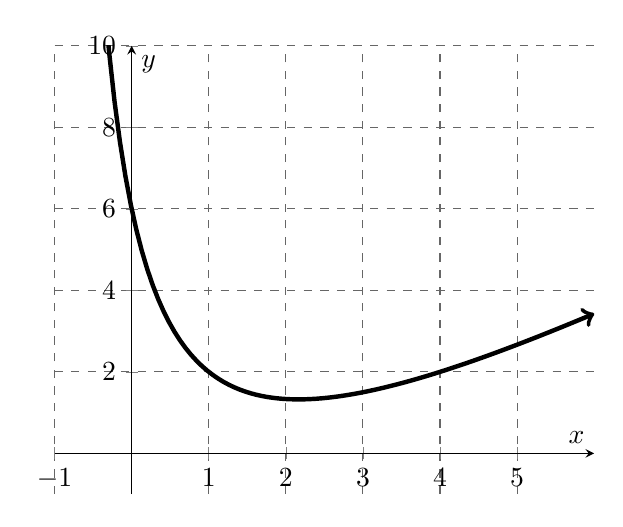
\begin{tikzpicture}
 \begin{axis}[
    xmin = -1, xmax = 6,
    ymin = -1, ymax = 10, xtick={-1,0,...,5}, ytick={-2,0,...,10},
    grid=both, grid style={ thin, black!60, dashed},axis x line=middle, axis y line=
middle, xlabel={$x$}, ylabel={$y$}]
    \addplot[ultra thick, <->,samples=100,
        domain = -1:6,
    ] {10/(x+1)+x-4};
    %\addplot[thick,->] coordinates {(-1,0) (6,0)};
\end{axis}
\end{tikzpicture}

Left is a sketch of the graph of $$f(x)=\displaystyle{\frac{10}{x+1}+x-4}.$$ \\
Sketch and label the \emph{tangent} line to the graph at the point $P(0,6).$\\
Sketch and label the \emph{secant} line between $P(0,6)$ and $Q(4,f(4)).$
\end{multicols}
\end{subproblems}
\newpage

\problem{8} Evaluate the expressions below. Assume all angles are measured in radians.\\


\begin{subproblems}
\begin{multicols}{2}
	\item $\displaystyle \sin ( \pi /4)= $
	\item $\displaystyle \cos(7 \pi /6)=$
\end{multicols}
\vspace{1in}	
\begin{multicols}{2}
	\item $\displaystyle \tan (2 \pi /3)= $
	\item $\displaystyle \sin (- \pi /2) =$
\end{multicols}
\vspace{1in}
\end{subproblems}


\problem{2} Use the right triangle below, with side lengths 12, 5 and 13,  to evaluate the expressions.\\

\vspace{.1in}

\begin{multicols}{2}
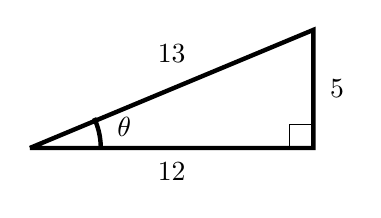
\begin{tikzpicture}[scale=0.3]
\draw[ultra thick] (0,0) -- (12,0) -- (12,5) -- (0,0);
\node at (6,-1){12}; 
\node at (13,2.5){5}; \node at (6,4){13};
\draw [ultra thick,domain=0:25] plot ({3*cos(\x)}, {3*sin(\x)});
\node at (4,.9){$\theta$};
\draw (11,0) -- (11,1) -- (12,1);
\end{tikzpicture}
\begin{subproblems}
\item $\displaystyle \cos (\theta) =$
\item $\displaystyle \csc (\theta) =$
\end{subproblems}
\end{multicols}
\vspace{.5in}

\problem{4} An athlete is running along a straight path. The position of the athlete is given by $d(t)=\frac{1}{2} t^2+t,$ where $t$ is time measured in seconds and $d$ is distance measured in meters. Find the average velocity of the athlete between $t=2$ and $t=4.$ Include units with your answer.
\vfill
	
\end{document}